\section{Iron---Berry curvature, anomalous Hall conductivity and optical conductivity}
\label{sec18:IronBerry}

\begin{itemize}
	\item Outline: {\it Calculate the Berry curvature, anomalous Hall conductivity, and (magneto)optical conductivity of ferromagnetic bcc Fe with spin-orbit coupling. In preparation for this example it may be useful to read Ref.~\onlinecite{PhysRevLett92} and Ch. 11 of the User Guide.}
\end{itemize}

\begin{itemize}
	\item[1-6] {\it Compute the MLWFs and compute the energy eigenvalues and spin expectation values.} 

	These are the same six steps of Ex.~\ref{sec17:IronSO} and therefore the results are not going to be showed here again.
\end{itemize}

\subsection*{Berry curvature plots}
\begin{itemize}
	\item {\it The Berry curvature $\Omega_{\alpha\beta}(\mathbf{k})$ of the occupied states is defined in Eq. (11.18) of the User Guide.}
	{\it Plot the Berry curvature component $\Omega_z(\bfk) = \Omega_{xy}(\bfk)$ along the magnetization direction.}

	The Fermi energy should be $12.6283$ eV. With this value we obtain the energy bands and the Berry curvature component $\Omega_z(\bfk) = \Omega_{xy}(\bfk)$ along high-symmetry points shown in \Fig{fig18.1} and \Fig{fig18.2}. Eq. (11.18) of the User Guide is reported below for completeness.

\begin{equation}
\Omega_{\alpha\beta}(\mathbf{k}) = \sum_{n}^{occ} f_{n\mathbf{k}}\Omega_{n,\alpha\beta},
\end{equation}
with
\begin{equation}
\Omega_{n,\alpha\beta} = \varepsilon_{\alpha\beta\gamma}\Omega_{n,\gamma} = -2\;\mathrm{Im}\braket{\nabla_{k_\alpha}\unk \vert \nabla_{k_\beta}\unk},
\end{equation}
where the Greek letters indicate Cartesian coordinates, $\varepsilon_{\alpha\beta\gamma}$ is the Levi-Civita antisymmetric tensor, and $\ket{u_{n\bfk}}$s 
are the cell-periodic Bloch functions.
\end{itemize}

\begin{figure}[b!]
\centering
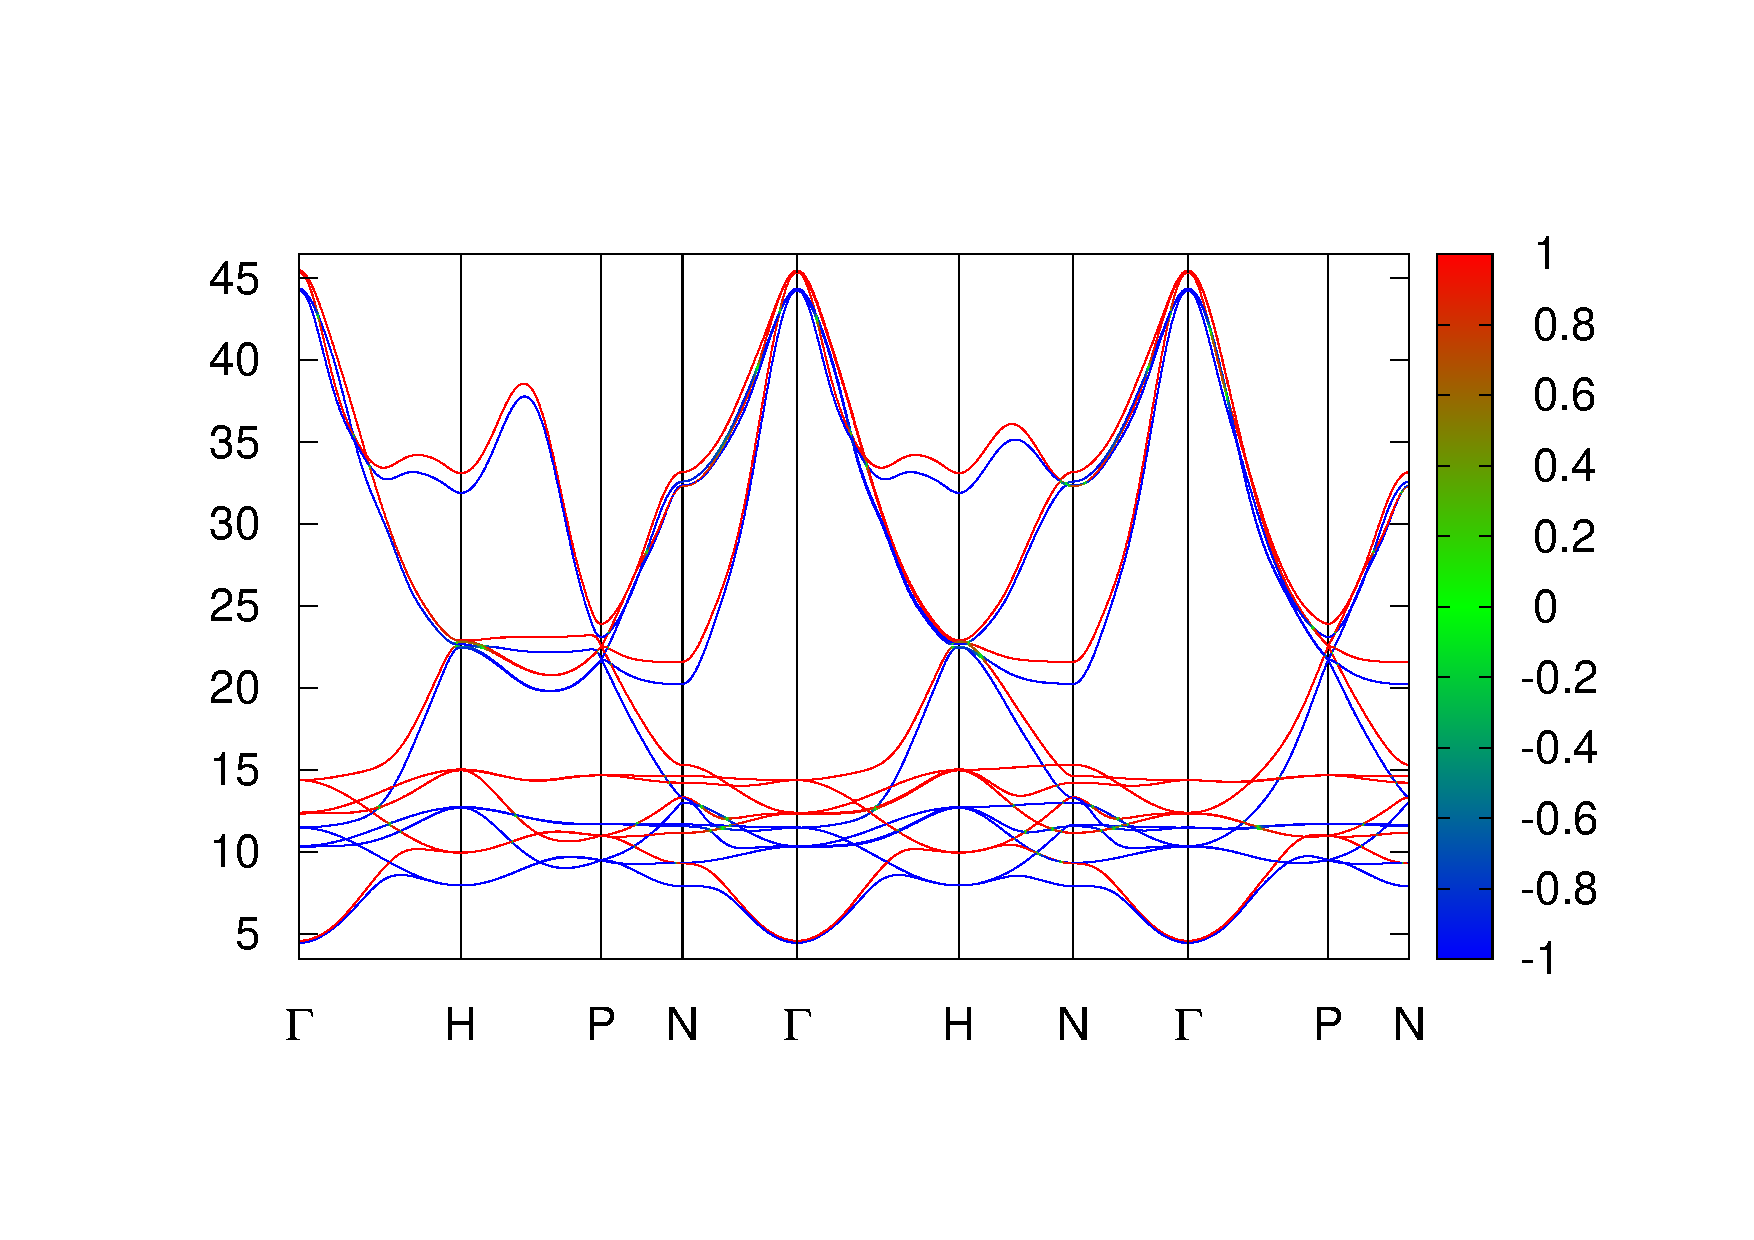
\includegraphics[width=0.8\columnwidth,trim={50pt 80pt 50pt 80pt},clip]{figure/example18/Fe_bandstructure.pdf}
\caption{Band structure of Fe along symmetry lines $\Gamma$-H-P-N-$\Gamma$-H-N-$\Gamma$-P-N.}
\label{fig18.1}
\end{figure}
\clearpage

\begin{figure}[t!]
\centering
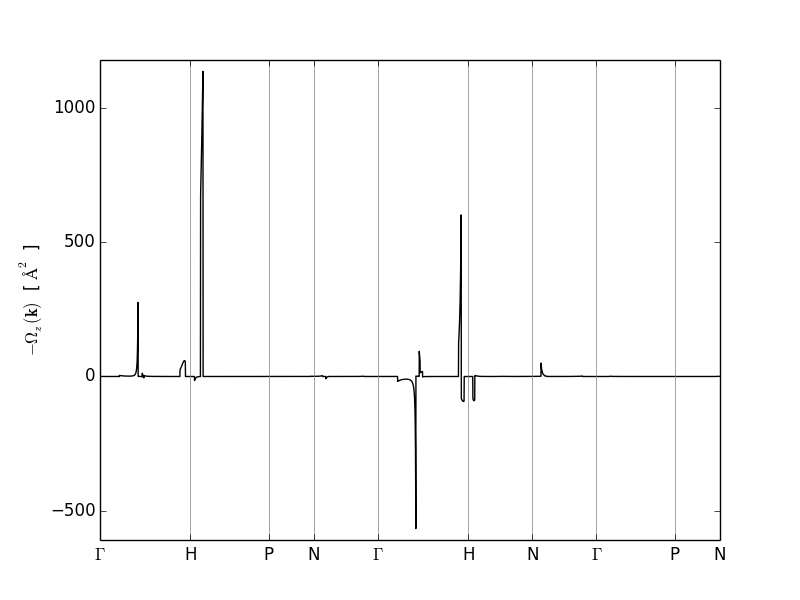
\includegraphics[width=0.7\columnwidth]{figure/example18/Fe_Berry_phase.png}
\caption{Berry curvature $\Omega_z(\bfk)$ in Fe along symmetry lines.}\label{fig18.2}
\end{figure}

\begin{itemize}
	\item {\it Combine the plot of the Fermi lines on the $k_y$ plane with a heatmap plot of (minus) the Berry curvature}

	The plot of the Fermi lines with a colormap of $-\Omega_z(k_x,0,k_z)$ is shown in \Fig{fig18.2}.
\end{itemize}

\begin{figure}[b!]
\centering
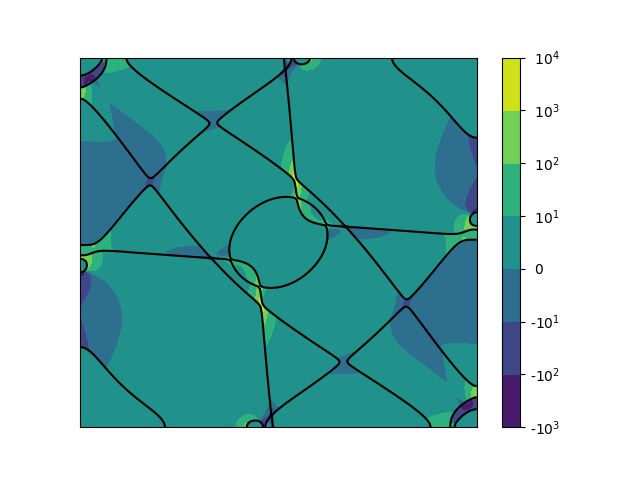
\includegraphics[width=0.5\columnwidth]{figure/example18/Fe_Fermi_surface+Berry_phase.png}
\caption{(Color online) Calculated total Berry curvature $−\Omega_z(\bfk)$ in the plane $k_y=0$ (note log scale). Intersections of the Fermi surface
with this plane are shown.}\label{fig18.3}
\end{figure}

\subsection*{Anomalous Hall conductivity}

\begin{itemize}
	\item {\it AHC converges rather slowly with k-point sampling, and a 25 × 25 × 25 does not yield a well-converged value.
	Compare the converged AHC value with those obtained in Refs.~\onlinecite{PhysRevB74} and \onlinecite{PhysRevLett92}.}

	The {\it x,y,z}-components of the AHC for a $25\times25\times25$ BZ mesh are shown in the snippet below. The converged result reported in Refs.~\onlinecite{PhysRevB74} and \onlinecite{PhysRevLett92} for the \textit{z}-component is 756.76 ($(\Omega \mathrm{cm})^{-1}$). Hence, a $25\times25\times25$ BZ mesh clearly gives a very inaccurate value ($\sim 36.4\%$ error). Even with adaptive refinement the error is still very large ($\sim 31.7\%$). It is worth to note that the adaptive refinement slightly breaks the symmetry and gives non-zero values for the \textit{x}-component and \textit{y}-component, although these are opposite in sign.  

\begin{tcolorbox}[title=Without adaptive refinement,sharp corners,boxrule=0.5pt]
{\small
\begin{verbatim}
 Properties calculated in module  b e r r y
 ------------------------------------------

   * Anomalous Hall conductivity
  
 Interpolation grid: 25 25 25

 Fermi energy (ev):   12.6283

 AHC (S/cm)       x          y          z
 ==========    -0.0000     0.0000   554.6437


 Total Execution Time          59.112 (sec)

\end{verbatim}
}
\end{tcolorbox}

\begin{tcolorbox}[title=With adaptive refinement,sharp corners,boxrule=0.5pt]
{\small
\begin{verbatim}
 Properties calculated in module  b e r r y
 ------------------------------------------

   * Anomalous Hall conductivity
  
 Regular interpolation grid: 25 25 25
   Adaptive refinement grid: 5 5 5
       Refinement threshold: Berry curvature >100.00 bohr^2
  Points triggering refinement:   42( 0.27%)

 Fermi energy (ev):   12.6283

 AHC (S/cm)       x          y          z
 ==========     2.4602    -2.4602   574.2950
\end{verbatim}
}
\end{tcolorbox}

Since these are quite demanding calculations, we only report the value of the AHC for a $125\times125\times125$ BZ mesh with a $5\times5\times5$ adaptive refinement grid (see snippet below). The value for the \textit{z}-component is 729.8276 $(\Omega \mathrm{cm})^{-1}$, which is in much closer agreement with the converged result from Refs.~\onlinecite{PhysRevB74} and \onlinecite{PhysRevLett92}. Also, the magnituted of \textit{x,y}-component is greatly reduced as expected. 

\begin{tcolorbox}[title={$125\times125\times125$ BZ mesh with a $5\times5\times5$ adaptive refinement grid}]
{\small
\begin{verbatim}
 Properties calculated in module  b e r r y
 ------------------------------------------

   * Anomalous Hall conductivity
  
 Regular interpolation grid: 125 125 125
   Adaptive refinement grid: 5 5 5
       Refinement threshold: Berry curvature >100.00 Ang^2
  Points triggering refinement: 1818( 0.09%)

 Fermi energy (ev):   12.6283

 AHC (S/cm)       x          y          z
 ==========    -0.2775     0.2775   729.8276
\end{verbatim}
}
\end{tcolorbox} 
\end{itemize}

\begin{itemize}
	\item {\it The Wannier-interpolation formula for the Berry curvature comprises three terms, denoted $J0$, $J1$, and $J2$ in Ref.~\onlinecite{PhysRevB85}.}

From Ref.~\onlinecite{PhysRevB74}
\begin{equation}
-2\;\mathrm{Im} G_{\alpha\beta} = J0 + J1 + J2, 
\end{equation}
where 
\begin{equation}
G_{\alpha\beta} = Tr[(\partial_\alpha \hat{P})\hat{Q}\hat{H}\hat{Q}(\partial_\beta\hat{P})]
\end{equation}

The three components $J0, J1$ and $J2$ for the $k$-point sampling of $125\times125\times125$ and a $5\times5\times5$ adaptive refinement grid are shown in the snippet below 
\end{itemize}
\begin{tcolorbox}[sharp corners,boxrule=0.5pt]
{\small
\begin{verbatim}
 J0 term :      0.0002    -0.0002     2.8479
 J1 term :      0.0004    -0.0004    18.4855
 J2 term :     -0.2782     0.2782   708.4942
 -------------------------------------------
\end{verbatim}
}
\end{tcolorbox}

\subsection*{Optical conductivity}
\begin{itemize}
	\item {\it The optical conductivity tensor of bcc Fe with magnetization along $\hat{\mathbf{z}}$ has the form }
\begin{equation}
\boldsymbol{\sigma} = \boldsymbol{\sigma}_\mathrm{S} + \boldsymbol{\sigma}_{\mathrm{A}} = 
\begin{pmatrix} 
\sigma_{xx} & 0                       & 0 \\ 
 0          & \sigma_{yy}=\sigma_{xx}  & 0 \\ 
 0          &  0                     & \sigma_{zz} 
\end{pmatrix} + \begin{pmatrix} 0 & \sigma_{xy} & 0 \\ -\sigma_{yx} & 0 & 0 \\ 0 & 0 & 0 \end{pmatrix} 
\end{equation}

	\item {\it
The dc AHC calculated earlier corresponds to $\sigma_{xy}$ in the limit $\omega \rightarrow 0$. At finite frequency $\sigma_{xy} = -\sigma_{yx}$ acquires
an imaginary part which describes magnetic circular dichoism (MCD).
Compute the complex optical conductivy for $\hbar\omega$ up to $7$ eV
}

The plot for the ac AHC is shown in \Fig{fig18.4}.

\end{itemize} 
\begin{figure}[t!]
\centering
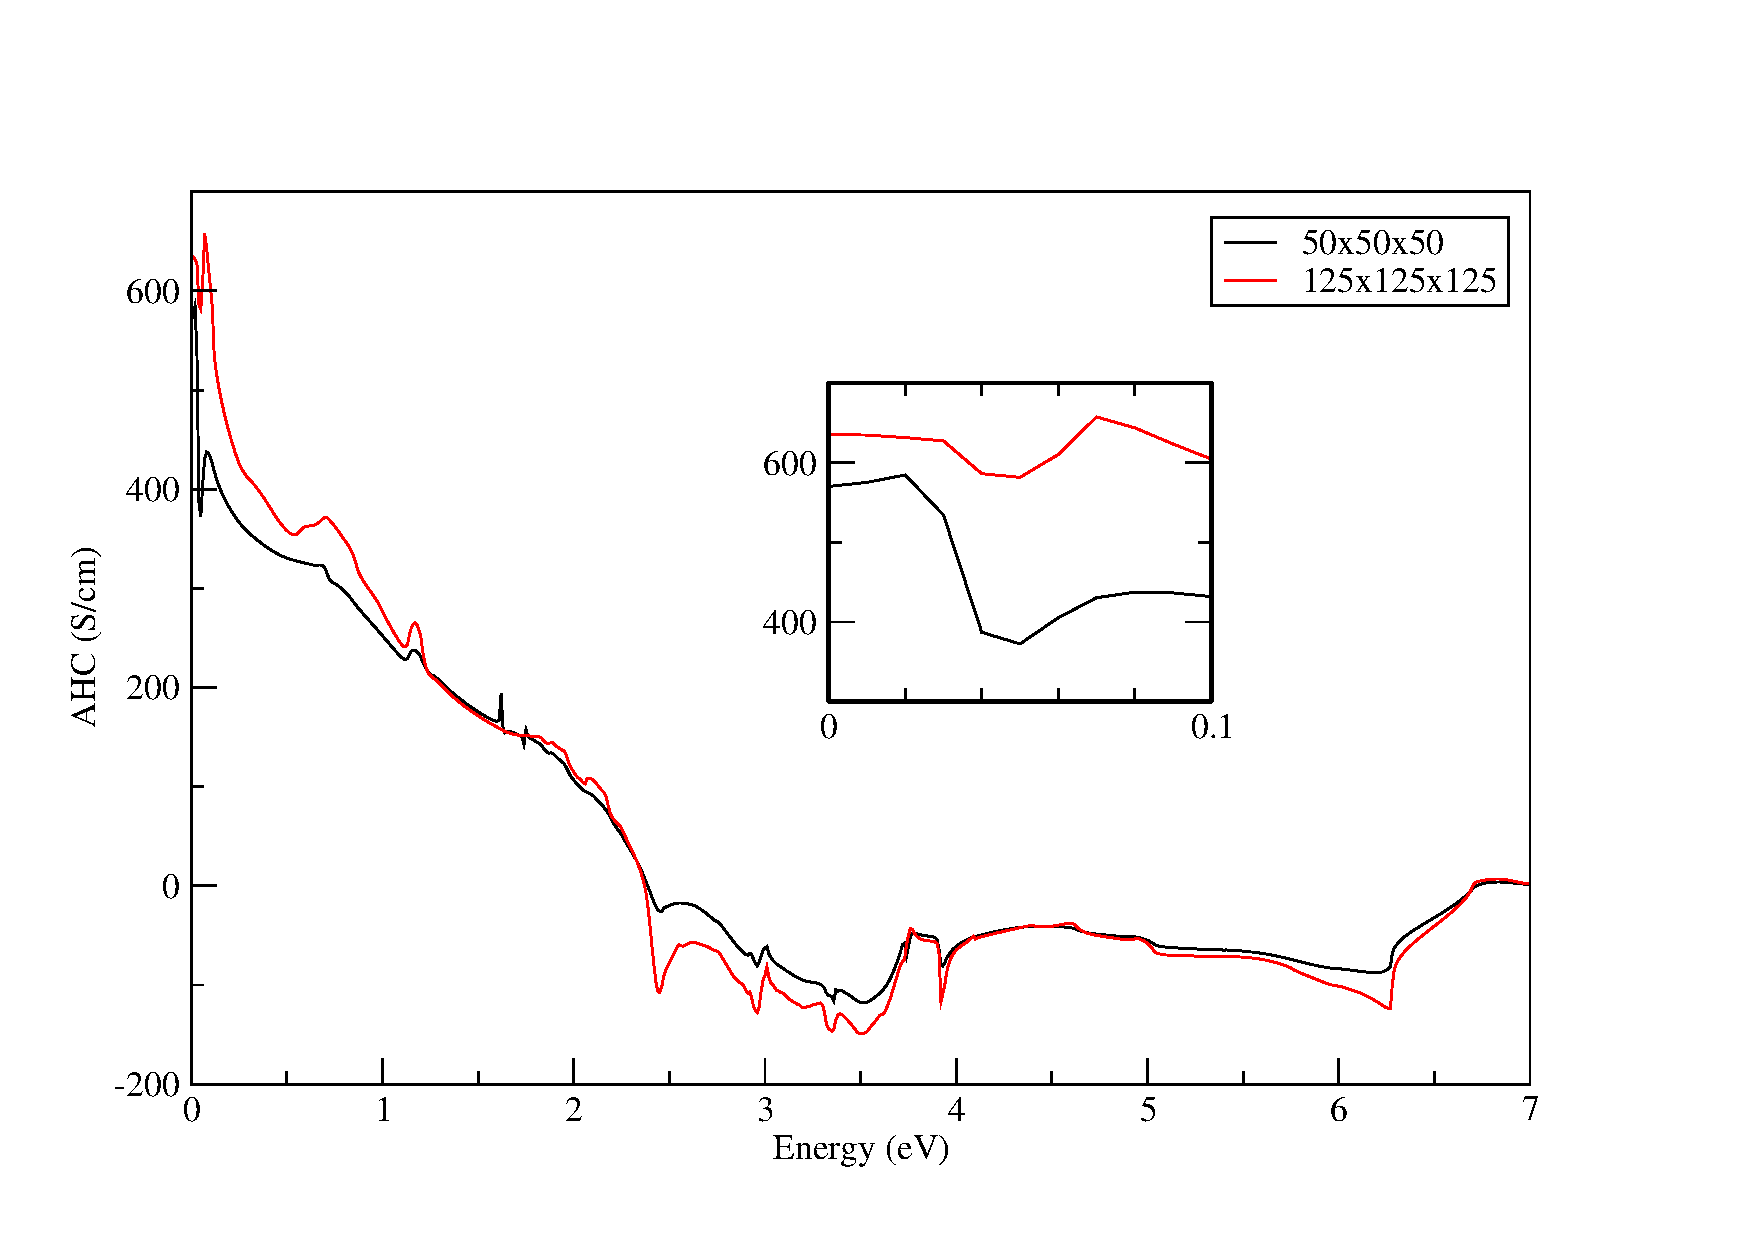
\includegraphics[width=0.7\columnwidth]{figure/example18/Fe-kubo_A_xy_125.pdf}
\caption{Plot of the real part of the complex optical conductivity with a $50\times50\times50$ $k$-point mesh (black) and $125\times125\times125$ $k$-point mesh (red). The inset is a magnification of the region [0-0.1] eV.}\label{fig18.4}
\end{figure}

\begin{itemize}
	\item {\it Comapare the $\omega \rightarrow 0$ limit of $\sigma_{xy}$ with the result obtained earlier by integrating the Berry curvature.}

	The result obtained by integrating the Berry curvature is 729.83 $(\Omega \mathrm{cm})^{-1}$ and the $\omega \rightarrow 0$ limit of the complex optical conductivity is $669.37$ $(\Omega \mathrm{cm})^{-1}$.

    {\it Plot the MCD spectrum.}

    The plot of the magnetic circular dichroism is shown in \Fig{fig18.5}.
\end{itemize}

\begin{figure}[t!]
\centering
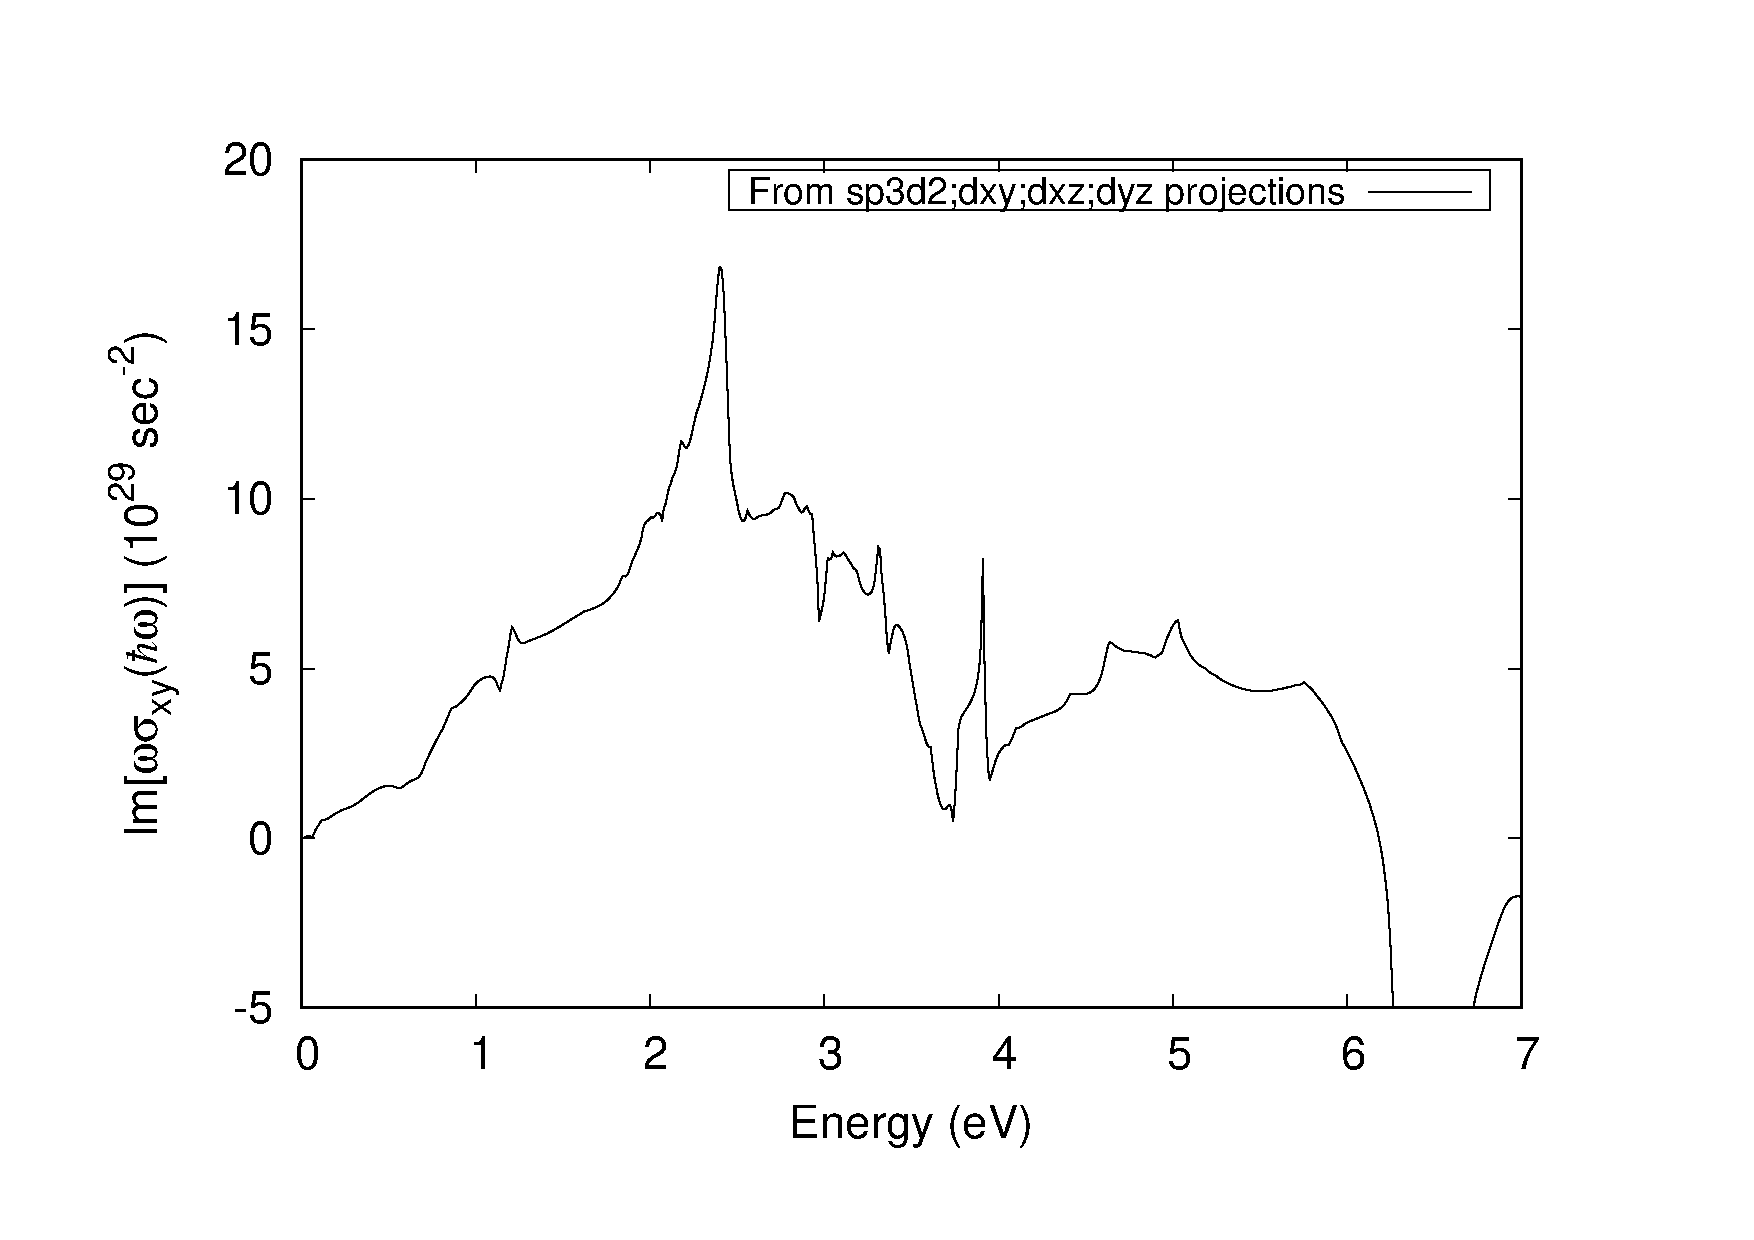
\includegraphics[width=0.7\columnwidth]{figure/example18/Fe_MCD_xy_125_sp3d2_projections.pdf}
\caption{The magnetic circular dicrhoism from interpolation of the Kubo-Greenwood formula.}
\label{fig18.5}
\end{figure}
\clearpage
\subsection*{Further ideas}
\begin{itemize}
	\item {\it Recompute the AHC and optical spectra of bcc Fe using projected s, p, and d-type Wannier
functions instead of the hybridrized MLWFs (see Example 8), and compare the results.}

First we have to modify the projection block in the input file {\tt Fe.win} as did in Ex.~\ref{sec8:Iron}

{\tt
\begin{quote}
begin projections
Fe:s;p;d
end projections
\end{quote}
}

Then we need to re-do points 3,4 and 6.

Below there is the extract from the output file {\tt Fe.wpout}. The result obtained from $s,p$ and $d$ projections for the $z$ component, i.e. $\sigma_{xy}$, of the AHC is exactly the same as the one obtained from $sp_3d_2,d_{xy},d_{xz}$, and $d_{yz}$ projections. Plot of AHC and MCD are shown in \Fig{fig18.6}.
	{\small
	\begin{tcolorbox}[title=With adaptive refinement,sharp corners,boxrule=0.5pt]
	\begin{verbatim}
 Properties calculated in module  b e r r y
 ------------------------------------------

   * Anomalous Hall conductivity
  
 Regular interpolation grid: 25 25 25
   Adaptive refinement grid: 5 5 5
       Refinement threshold: Berry curvature >100.00 bohr^2
  Points triggering refinement:   42( 0.27%)

 Fermi energy (ev):   12.6283

 AHC (S/cm)       x          y          z
 ==========
 J0 term :      0.0006    -0.0006    -2.9033
 J1 term :      0.0032    -0.0032    10.0566
 J2 term :      2.4564    -2.4564   567.1417
 -------------------------------------------
 Total   :      2.4602    -2.4602   574.2950

	\end{verbatim}
	\end{tcolorbox}
	}

\begin{figure}[b!]
\centering
\subfloat[AHC]{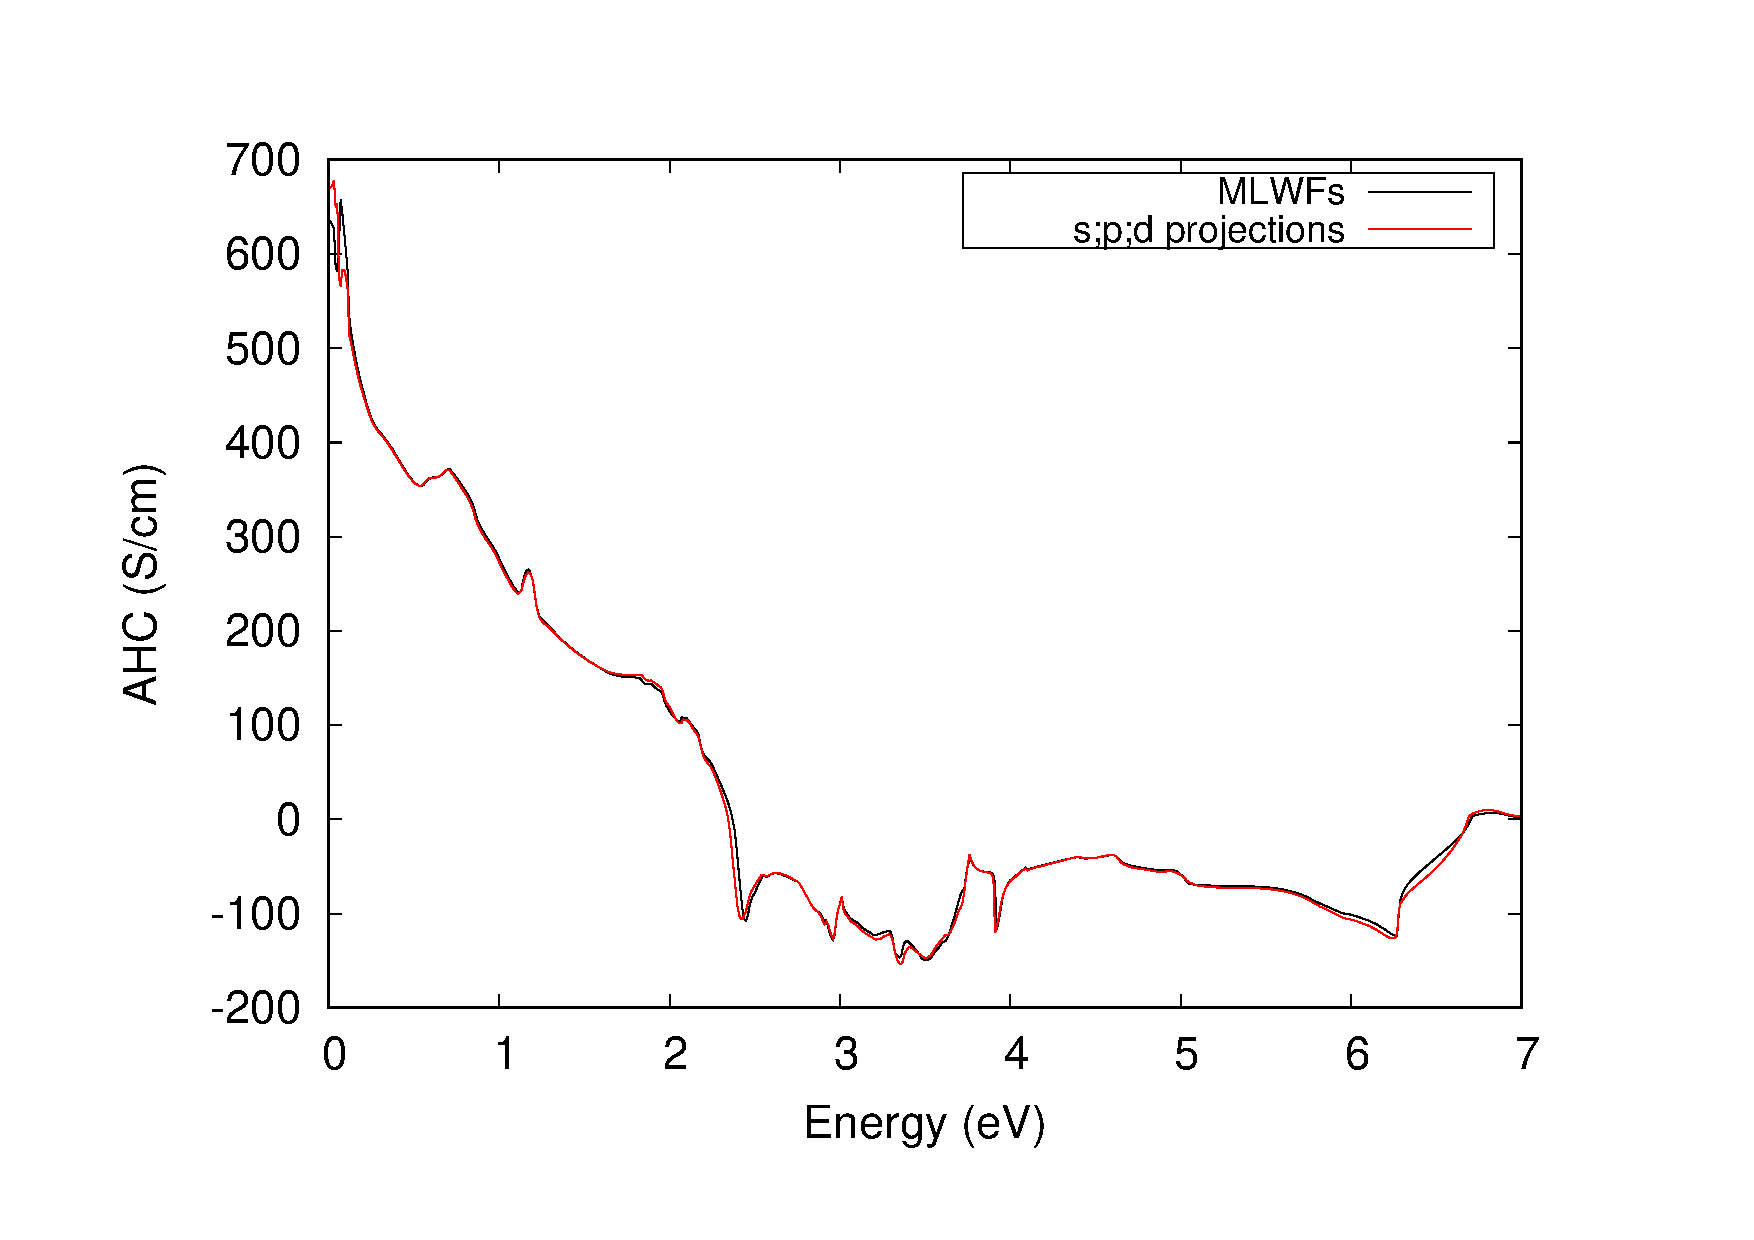
\includegraphics[width=0.5\columnwidth]{figure/example18/Fe_optical_conductivity_xy_125_MLWFs_and_projections.pdf}}
\centering
\subfloat[MCD]{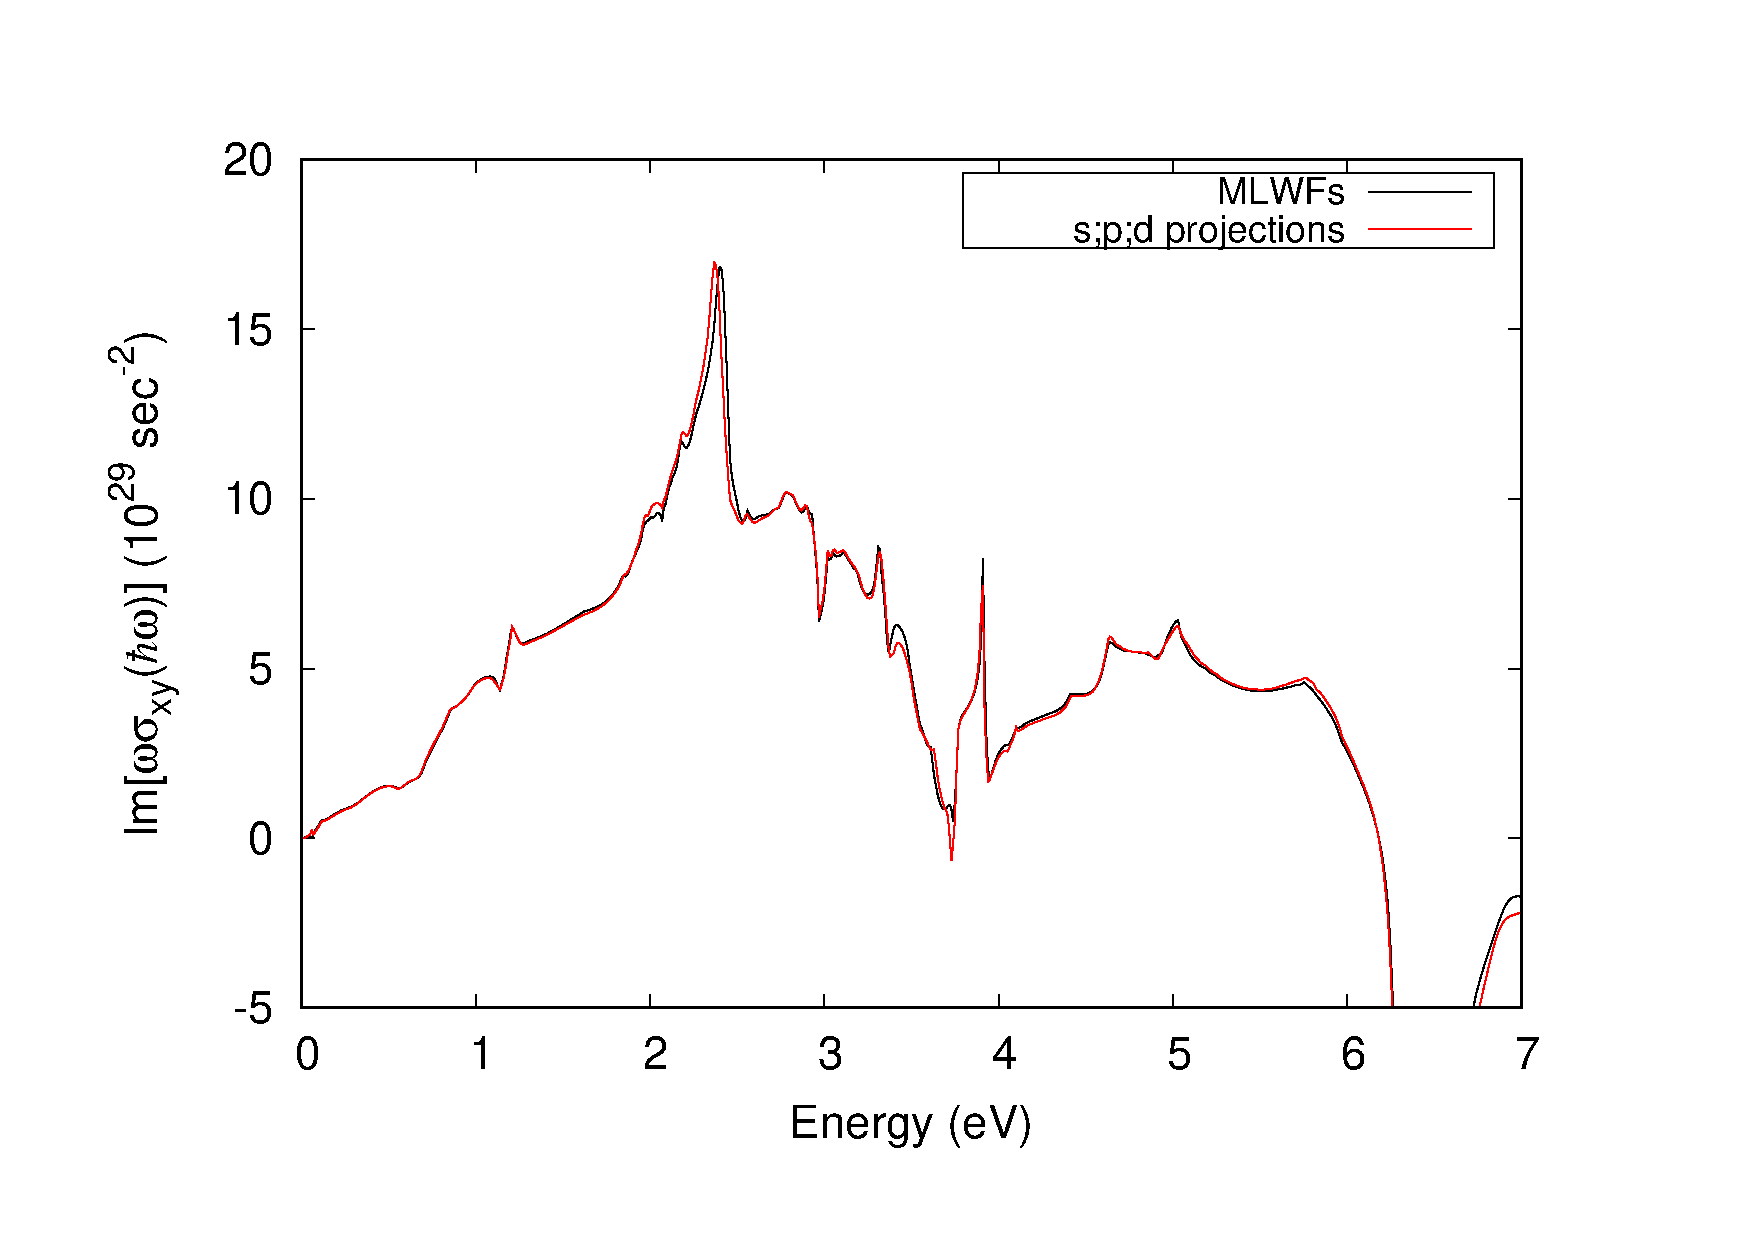
\includegraphics[width=0.5\columnwidth]{figure/example18/Fe_MCD_xy_125_MLWFs_and_projections.pdf}}
\caption{Left panel: Anomalous Hall conductivity. Right panel: Magnetic circular dichroism for $\hbar\omega$ up to $7$ eV, starting from $s;p;d$ initial projections}\label{fig18.6}
\end{figure}

\end{itemize}
